\chapter{Nadajnik ultradźwiękowy}
\section{Budowa i zasada działania}

Nadajnik zbudowany został w oparciu o \textit{Arduino Nano} \cite{bib:arduinoNano} do którego podłączono 
bezpośrednio cztery nadajniki ultradźwiękowe (rezonatory piezoelektryczne) typu 40ST-12 \cite{bib:40ST12}, schemat 
przedstawiony jest na rysunku \ref{fig:nadajnik_schemat}.

\rysunek{transmitter}{schemat nadajnika ultradźwiękowego}{\label{fig:nadajnik_schemat}}


Całość umieszczona została w ramie w kształcie litery \textbf{H} wykonanej z rurek PCV.
Rezonatory zostały dodatkowo odizolowane od ramy rzepami co ułatwia ich zdejmowanie jak i skutecznie
zapobiega przenoszeniu się drgań.

\rysunek{nadajnik_H}{szkic ramy nadajnika}{\label{fig:nadajnik_szkic}}


Android Nano połączony jest z odbiornikiem 6m kablem, którym przesyłane są sygnały sterujące jak i zasilanie.
Do sterowania wykorzystywane są trzy przewody, dwa z nich informują który z rezonatorów ma w danym momencie nadawać,
trzeci służy jako wyzwalacz. 

Cała logika oprogramowania mieści się w obsłudze przerwania sprzętowego, które reaguje na zmianą stanu logicznego
na wyzwalaczu,
po uruchomieniu przerwania oprogramowanie wysyła sygnał na odpowiedni rezonator. 
Nadawany sygnał jest tak dobrany by dało się go w prosty sposób wyodrębnić i składa się w dwóch
części: część wzbudzającej oraz części tłumiącej.
Długość impulsów sygnału jest zgodna z częstotliwością rezonansową nadajników, dodatkowo część tłumiąca
jest przesunięty względem części wyzwalającej o 180 stopni.  
Rysunek \ref{fig:output_signal} przedstawia sygnał jakim wysterowany jest przetwornik piezoelektryczny. 

Odległość między nadajnikiem a odbiornikami wyznaczany jest przez odbiornik na podstawie
czasu jaki potrzebował sygnał dźwiękowy by do niego dotrzeć.

 \begin{figure}[h!]
    \centering
    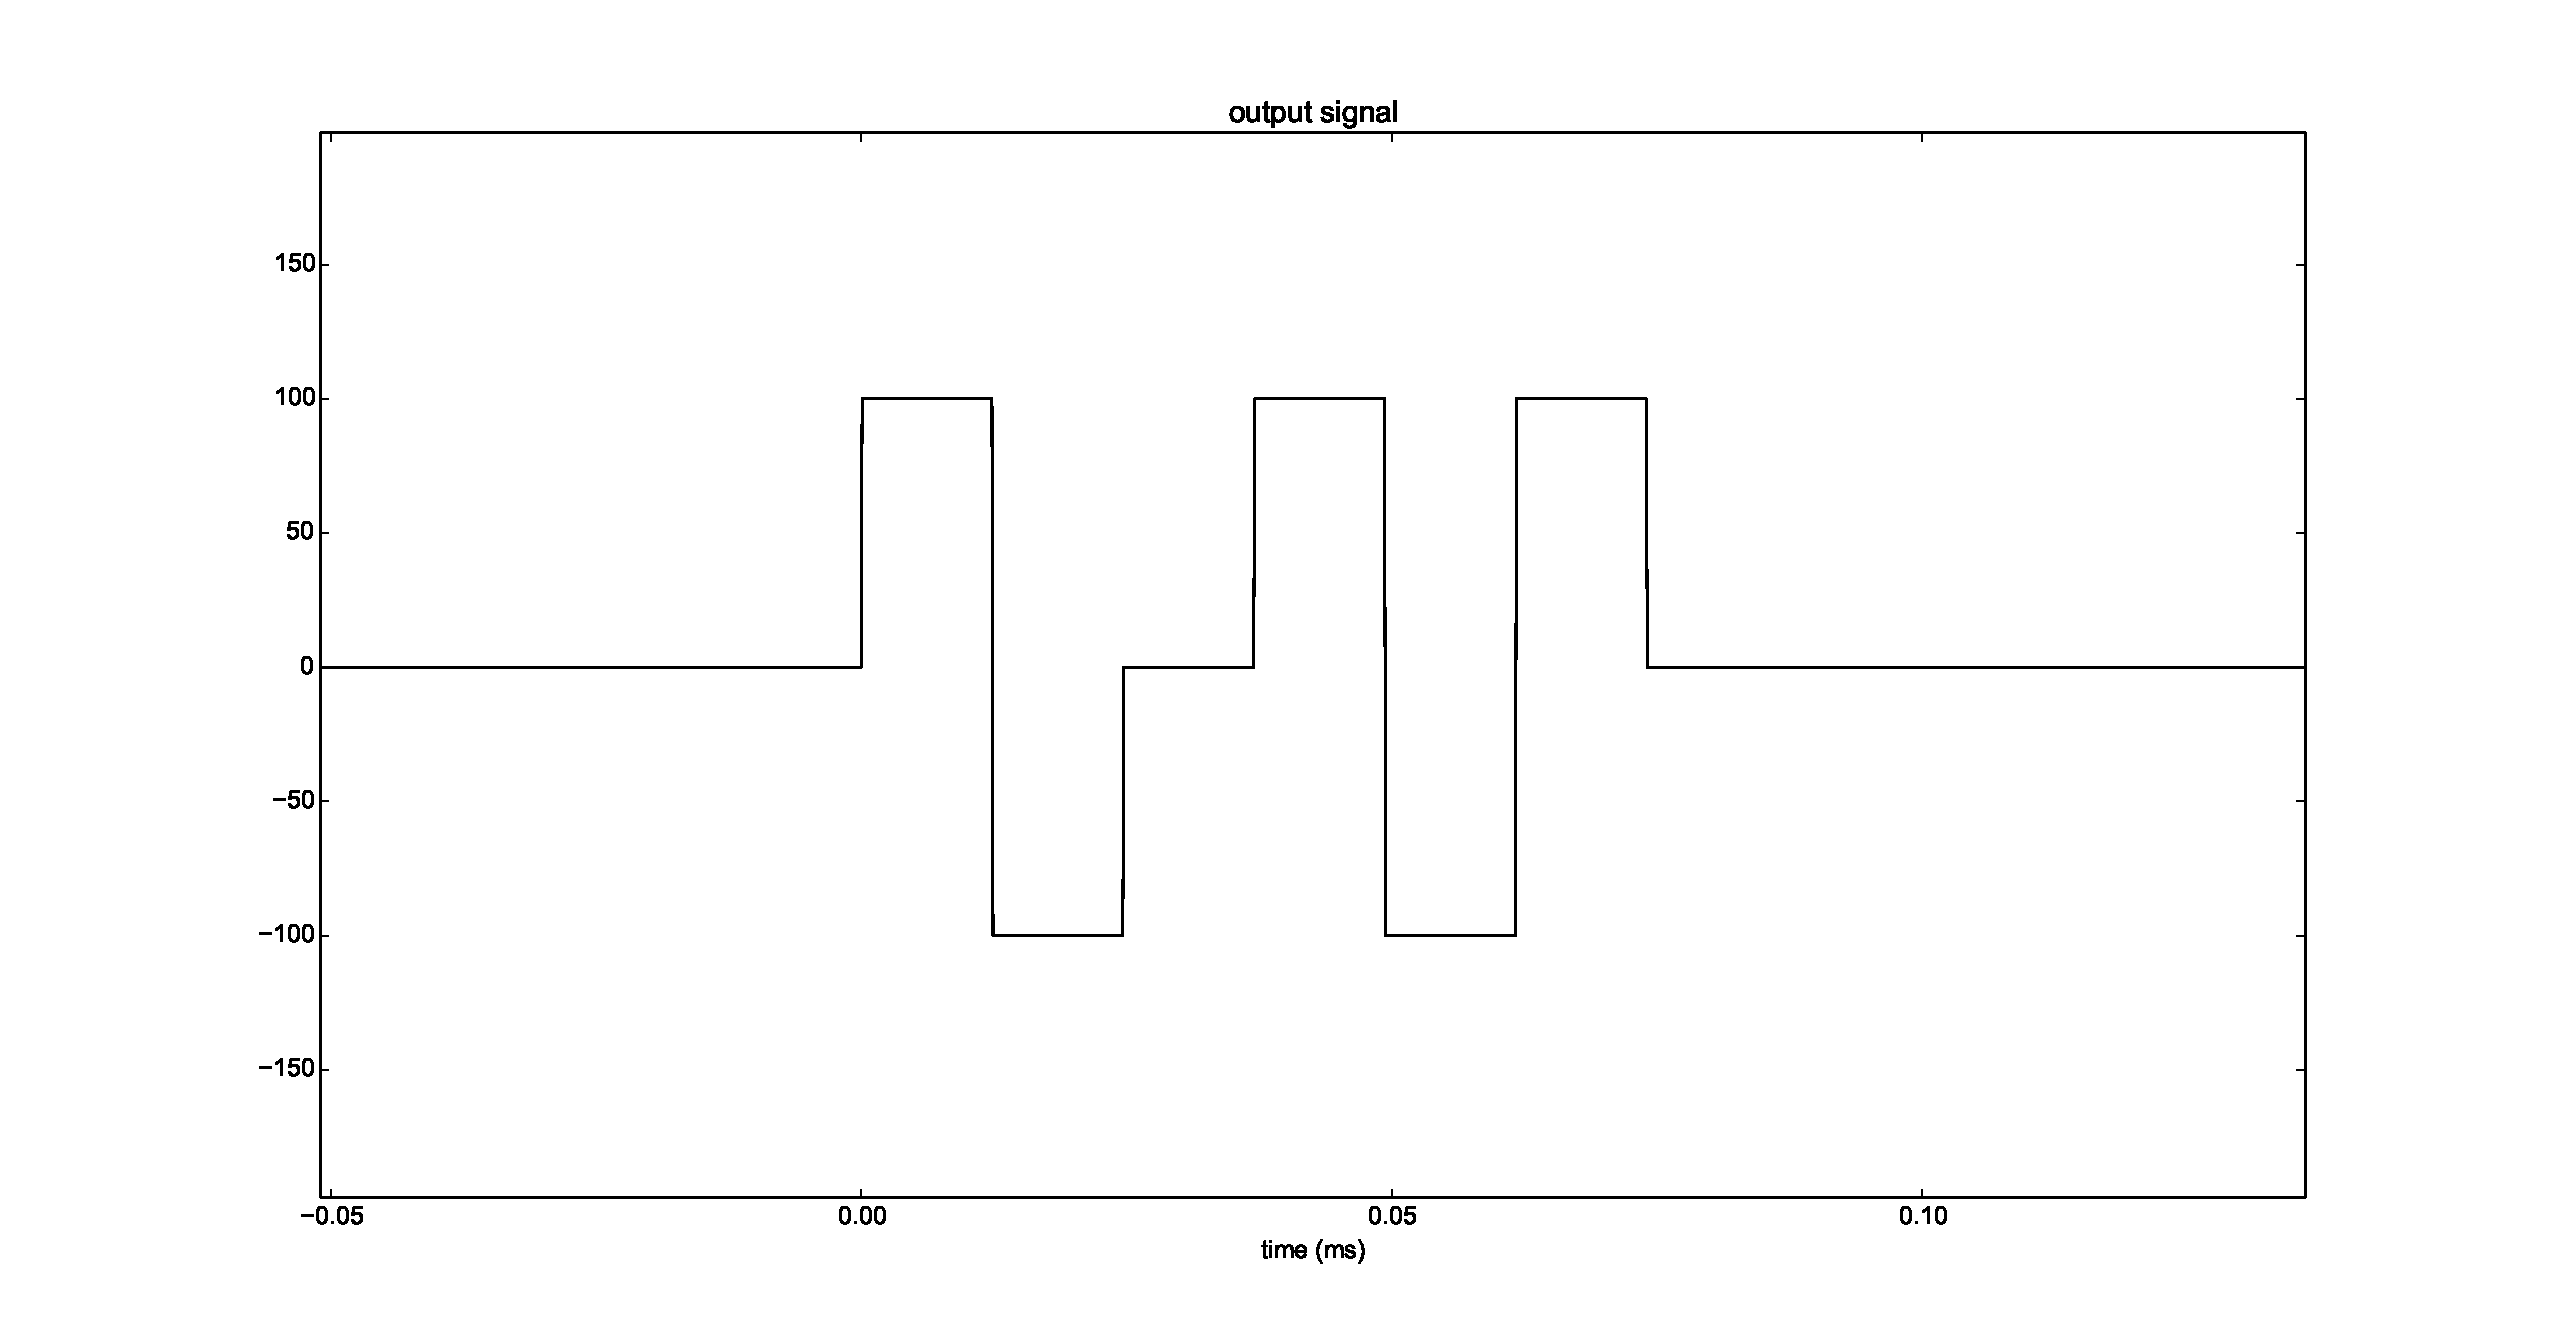
\includegraphics[width=1.15\textwidth, trim= 47mm 0mm 0mm 0mm,clip]{output_signal}
    \caption{sygnał wysterowania nadajnika piezoelektrycznego}
    \label{fig:output_signal}
\end{figure}

\newpage

\section{Dobór rezonatorów piezoelektrycznych}

Głównym problemem podczas konstrukcji nadajnika okazał się dobór odpowiednich rezonatorów piezoelektrycznych.
Mimo, że producent zapewnia zakres pracy rezonatorów w zakresie: $40 kHz \pm 1kHz$, taki rozrzut okazał się niewystarczający, 
dlatego z 30 rezonatorów (15 nadajników i 15 odbiorników) wybrane zostały 4 nadajniki i 3 odbiorniki o najbardziej 
zbliżonych częstotliwościach pracy. Częstotliwości zostały zmierzone na oscyloskopie cyfrowym, są to odpowiedzi 
rezonatora na krótki impuls elektryczny.

Tabela \ref{table:czestotliwosci} zawiera wyniki pomiarów częstotliwości, gwiazdką oznaczono wykorzystane przetworniki piezoelektryczne.

\begin{table}[t]
  \centering
  \begin{tabular}{|r|r|r|}
    \hline 
    Nr & Nadajnik: 40ST-12 & Odbiornik: 40SR-12\\
    \hline
    1  &   \SI{40,88}{kHz} & *\SI{40,65}{kHz} \\
    2  &   \SI{41,12}{kHz} &  \SI{40,45}{kHz} \\
    3  &  *\SI{40,78}{kHz} &  \SI{39,52}{kHz} \\
    4  &   \SI{41,19}{kHz} &  \SI{40,47}{kHz} \\
    5  &   \SI{40,92}{kHz} &  \SI{40,66}{kHz} \\
    6  &   \SI{39,68}{kHz} & *\SI{40,69}{kHz} \\
    7  &   \SI{39,78}{kHz} &  \SI{40,59}{kHz} \\
    8  &  *\SI{40,80}{kHz} &  \SI{40,39}{kHz} \\
    9  &   \SI{40,90}{kHz} &  \SI{40,29}{kHz} \\
    10 &  *\SI{40,66}{kHz} & *\SI{40,68}{kHz} \\
    11 &  *\SI{40,85}{kHz} &  \SI{39,22}{kHz} \\
    12 &   \SI{41,01}{kHz} &  \SI{39,51}{kHz} \\
    13 &   \SI{41,00}{kHz} &  \SI{39,92}{kHz} \\
    14 &   \SI{39,82}{kHz} &  \SI{39,26}{kHz} \\
    15 &   \SI{39,64}{kHz} &  \SI{39,11}{kHz} \\
    \hline
  \end{tabular}
  \caption{Częstotliwości rezonansowe przetworników piezoelektrycznych}
  \label{table:czestotliwosci}
\end{table}


